\chapter{Technologie cible et outils}\label{chap:met}
Au cours des premières semaines du projet, l'un des objectifs qui nous était proposé était d'étudier le framework \play{} et de s'assurer de la compatibilité de sa philosophie avec un projet de génération de code. Dans la section \ref{sec:pla} de ce chapitre, nous détaillerons les qualités de ce framework qui ont motivées la sélection de \play{} pour ce projet. Dans un second temps (\cf{} section \ref{sec:pro}, nous aborderons le prototype que nous avons élaboré avec \play. 


\section{Framework Play}\label{sec:pla}
\play{} est un framework basé sur les langages Java et Scala permettant de la création d'applications web. De plus en plus de développeurs choisissent ce nouvel outil qui présente de nombreux avantages. L'aspect \og prêt à l'emploi \fg{} (\textit{Plug'n Play}) permis par ses fonctionnalités par défaut le rendent efficace et rapide d'utilisation. Le développement est facilité, d'une part par par des mécanismes de compilation à la volée (\textit{shadow-build}), mais aussi par la mise à disposition de systèmes tests intégrées (JUnit, Selenium). La gestion des native des requêtes rendent ces dernières non-bloquantes (synchronisme). Enfin son architecture modulaire, composée de plugins et d'un \textit{design pattern} MVC, permettent une répartition claire du code source ce qui est propice à la démarche MDA.

{\huge $\Uparrow$ woua c'est nuull refractoring!!}



\section{Conception d’une maquette d’exemple}\label{sec:pro}

Le prototype proposé est une implémentation d'un site marchand. 

\begin{figure}[htb]
  \centering
  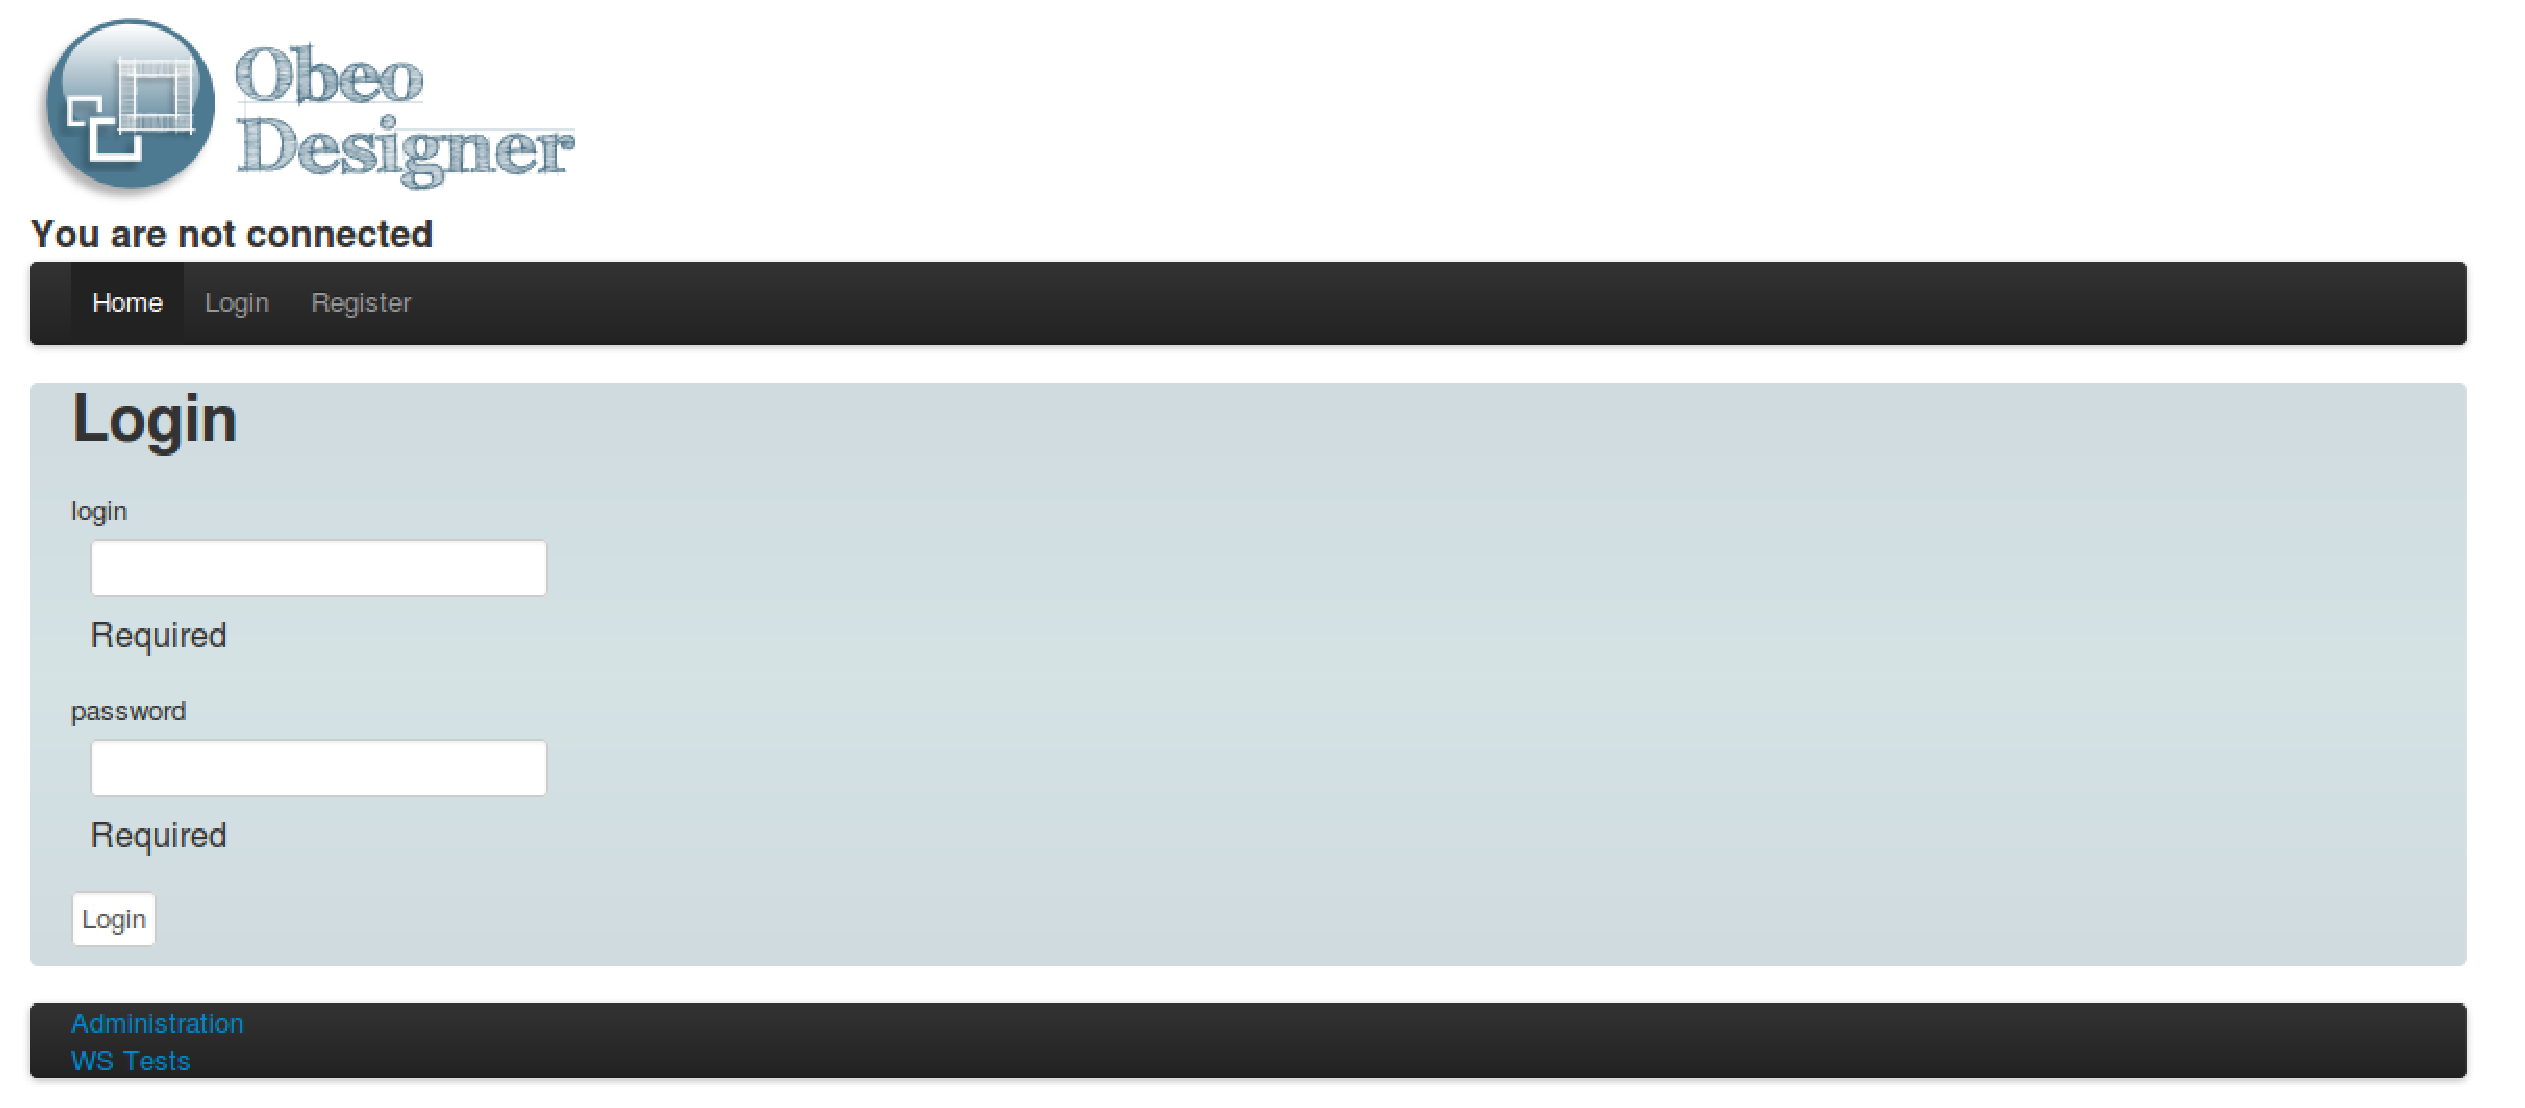
\includegraphics[scale=.2]{img/proto.eps}
  \caption{Prototype Play\_Shop}
  \label{fig:pro}
\end{figure}



%% \begin{figure}[htb]
%%   \centering
%%   \includegraphics[scale=.3]{img/Cin.eps}
%%   \caption{Méta model SOA}
%%   \label{fig:soa}
%% \end{figure}


%%  LocalWords:  framework play Scala web Plug'n shadow-build JUnit
%%  LocalWords:  Selenium non-bloquantes plugins MVC MDA woua nuull
%%  LocalWords:  refractoring implémentation Shop models Model Entity
%%  LocalWords:  méta-modèle model SOA blah bklah fdslmk
